Cet exercice est inspir{\'e} d'un probl{\`e}me de l'Olympiade Internationale de Math{\'e}matiques (IMO) 2021. Il s'agit d'un d{\'e}fi combinatoire o{\`u} vous devrez utiliser des raisonnements arithm{\'e}tiques et logiques pour r{\'e}soudre un probl{\`e}me de partition de cartes.

\begin{exercise}[(Probl{\`e}me 1 IMO 2021 Jour 1)]
Soit $n \geqslant 100$ un entier. Ivan {\'e}crit les nombres $n, n + 1,
\ldots, 2 n$ chacun sur une carte diff{\'e}rente. Il m{\'e}lange ensuite ces
$n + 1$ cartes et les divise en deux tas. Montrez qu'au moins un des tas
contient deux cartes dont la somme des nombres est un carr{\'e} parfait.

\end{exercise}

\subsection*{Solution. (SABIR Ilyass)}
\addcontentsline{toc}{subsection}{Solution. (SABIR Ilyass)}


Nous g{\'e}n{\'e}ralisons ce probl{\`e}me en posant la question suivante :

\tmtextbf{G{\'e}n{\'e}ralisation du probl{\`e}me 1.}

Soit $r \in \mathbb{N}$ tel que $r \geqslant 1$, et soit $n \geqslant \frac{5
r^2}{2} + \frac{5 r}{2}$ un entier. Ivan {\'e}crit les nombres $n, n + 1,
\ldots, 2 n$ chacun sur une carte diff{\'e}rente. Il m{\'e}lange ensuite ces
$n + 1$ cartes et les divise en $2 r$ tas. Montrez qu'au moins un des tas
contient deux cartes dont la somme des nombres est un carr{\'e} parfait.

Remarquons que l'exerice est un cas particulier o{\`u} \tmtextbf{$r = 1$}.
Nous nous int{\'e}ressons maintenant {\`a} la r{\'e}solution de cette
g{\'e}n{\'e}ralisation.

Pour avoir deux cartes dans l'un des tas de sorte que la somme de leurs
nombres soit un carr{\'e} parfait, il est suffisant de montrer qu'il existe $r
+ 1$ cartes telles que la somme de chaque paire de ces cartes soit un
carr{\'e} parfait.

Soient $x_1, \ldots, x_{2 r + 1} \in \mathbb{N}$, et $a_1, \ldots, a_{2 r + 1}
\in \llbracket n, 2 n \rrbracket$ satisfaisant le syst{\`e}me d'{\'e}quations
suivant :
\begin{eqnarray*}
  a_1 + a_2 & = & x_1^2\\
  a_2 + a_3 & = & x^2_2\\
  & . & \\
  & . & \\
  & . & \\
  a_{2 r} + a_{2 r + 1} & = & {x^2_{2 r}} \\
  a_{2 r + 1} + a_1 & = & x^2_{2 r + 1}
\end{eqnarray*}


Pour conclure, il suffit de prouver que ce syst{\`e}me d'{\'e}quations admet
une solution (avec certaines conditions sur $x_1, \ldots, x_n$), o{\`u} les
inconnues sont $(a_1, \ldots, a_{r + 1}) \in \llbracket n, 2 n \rrbracket^{2 r
+ 1}$.

On a :
\[ \underset{\tmop{cyc}}{\sum} (a_1 + a_2) = \underset{\tmop{cyc}}{\sum} x^2_1
   = \overset{r + 1}{\underset{k = 1}{\sum}} x^2_k \]


Remarquons que :


\[ x_{2 r + 2} = x_1, x_{2 r + 3} = x_2, \ldots, x_{4 r + 2} = x_{2 r + 1} \]
\text{ }

et
\[ a_{2 r + 2} = a_1, a_{2 r + 3} = a_2, \ldots, a_{4 r + 2} = a_{2 r + 1} \]


On a pour tout $l \in \llbracket 0, r \rrbracket$
\begin{eqnarray*}
  \underset{k = 1}{\overset{2 r + 1}{\sum}} (- 1)^k (a_{k + l} + a_{k + l +
  1}) & = & \underset{k = 0}{\overset{r - 1}{\sum}} [(a_{2 k + l + 2} + a_{2 k
  + l + 3}) - (a_{2 k + l + 2} + a_{2 k + l + 1})] - (a_{2 r + l + 1} + a_{2 r
  + 2 + l})\\
  & = & \underset{k = 0}{\overset{r - 1}{\sum}} [a_{2 k + l + 3} - a_{2 k + l
  + 1}] - (a_{2 r + l + 1} + a_{2 r + 2 + l})\\
  & = & \underset{k = 0}{\overset{r - 1}{\sum}} [a_{2 (k + 1) + l + 1} - a_{2
  k + l + 1}] - (a_{2 r + l + 1} + a_{2 r + 2 + l})\\
  & = & a_{2 r + l + 1} - a_{l + 1} - (a_{2 r + l + 1} + a_{2 r + 2 + l})\\
  & = & - a_{2 r + 2 + l} - a_{l + 1}\\
  & = & - 2 a_{l + 1}
\end{eqnarray*}


Ainsi, pour tout $l \in \llbracket 0, r \rrbracket$,
\[ a_{l + 1} = \frac{1}{2} \underset{k = 1}{\overset{2 r + 1}{\sum}} (- 1)^{k
   - 1} (a_{k + l} + a_{k + l + 1}) = \frac{1}{2} \underset{k = 1}{\overset{2
   r + 1}{\sum}} (- 1)^{k - 1} x^2_{k + l} \]


Par translation, nous pouvons en conclure que pour tout $j \in \llbracket 1, r
+ 1 \rrbracket$,
\[ a_j = \frac{1}{2} \underset{k = 1}{\overset{2 r + 1}{\sum}} (- 1)^{k - 1}
   (a_{k + j - 1} + a_{k + j}) = \frac{1}{2} \underset{k = 1}{\overset{2 r +
   1}{\sum}} (- 1)^{k - 1} x^2_{k + j - 1} \]


Nous cherchons {\`a} trouver $(x_1, x_2, \ldots, x_{2 r + 1}) \in \mathbb{N}$,
satisfaisant :
\[ \frac{1}{2} \underset{k = 1}{\overset{2 r + 1}{\sum}} (- 1)^{k - 1} x^2_{k
   + j - 1} \in \llbracket n, 2 n \rrbracket \]


pour tout $j \in \llbracket 1, r + 1 \rrbracket$, o{\`u} $x_{2 r + 2} = x_1,
x_{2 r + 3} = x_2, \ldots, x_{4 r + 2} = x_{2 r + 1}$.

Pour minimiser la valeur de
\[ \frac{1}{2} \underset{k = 1}{\overset{2 r + 1}{\sum}} (- 1)^{k - 1} x^2_{k
   + j - 1} \]


pour tout $j \in \llbracket 1, r + 1 \rrbracket$, il est naturel de
consid{\'e}rer $x_1, x_2, \ldots, x_{2 r + 1}$ comme {\'e}tant
cons{\'e}cutifs.

Et en raison de la somme altern{\'e}e, et pour simplifier le calcul, nous
consid{\'e}rons $\alpha \in \mathbb{N}^{\star},$ tel que, pour tout $j \in
\llbracket 1, 2 r + 1 \rrbracket$
\[ x_j = \alpha + j - r \]


On a pour tout $j \in \llbracket 1, 2 r + 1 \rrbracket$
\begin{eqnarray*}
  a_j & = & \frac{1}{2} \underset{k = 1}{\overset{2 r + 1}{\sum}} (- 1)^{k -
  1} (\alpha + k + j - r - 1)^2\\
  & = & \frac{1}{2} \underset{k = 1}{\overset{2 r + 1}{\sum}} (- 1)^{k - 1}
  (\alpha^2 + 2 (k + j - r - 1) \alpha + (k + j - r - 1)^2) \\
  & = & \left( \frac{1}{2} \underset{k = 1}{\overset{2 r + 1}{\sum}} (- 1)^{k
  - 1} \right) \alpha^2 + \left( \underset{k = 1}{\overset{2 r + 1}{\sum}} (-
  1)^{k - 1} (k + j - r - 1) \right) \alpha + \frac{1}{2} \underset{k =
  1}{\overset{2 r + 1}{\sum}} (- 1)^{k - 1} (k + j - r - 1)^2\\
  & = & \frac{1}{2} \alpha^2 + \left( \underset{k = 1}{\overset{2 r +
  1}{\sum}} (- 1)^{k - 1} (k + j - r - 1) \right) \alpha + \frac{1}{2}
  \underset{k = 1}{\overset{2 r + 1}{\sum}} (- 1)^{k - 1} (k + j - r - 1)^2
\end{eqnarray*}


o{\`u}
\begin{eqnarray*}
  \underset{k = 1}{\overset{2 r + 1}{\sum}} (- 1)^{k - 1} (k + j - r - 1) & =
  & \underset{k = 1}{\overset{2 r + 1}{\sum}} (- 1)^{k - 1} k + (j - r - 1)
  \underset{k = 1}{\overset{2 r + 1}{\sum}} (- 1)^{k - 1}\\
  & = & \underset{k = 1}{\overset{r}{\sum}} [2 k - (2 k - 1)] + j - r - 1 +
  (2 r + 1)\\
  & = & \left( \underset{k = 1}{\overset{r}{\sum}} 1 \right) + j + r\\
  & = & 2 r + j
\end{eqnarray*}


et
\begin{eqnarray*}
  \frac{1}{2} \underset{k = 1}{\overset{2 r + 1}{\sum}} (- 1)^{k - 1} (k + j -
  r - 1)^2 & = & \frac{1}{2} \underset{k = 1}{\overset{2 r + 1}{\sum}} (-
  1)^{k - 1} (k^2 + 2 k (j - r - 1) + (j - r - 1)^2) \\
  & = & \frac{1}{2} \underset{k = 1}{\overset{2 r + 1}{\sum}} (- 1)^{k - 1}
  k^2 + (j - r - 1) \underset{k = 1}{\overset{2 r + 1}{\sum}} (- 1)^{k - 1} k
  \\
  + \frac{(j - r - 1)^2}{2} \underset{k = 1}{\overset{2 r + 1}{\sum}} (-
  1)^{k - 1}\\
  & = & \frac{1}{2} \underset{k = 1}{\overset{r}{\sum}} [(2 k)^2 - (2 k -
  1)^2] + (j - r - 1) r + \frac{(j - r - 1)^2}{2} + (2 r + 1)^2\\
  & = & \frac{1}{2} \underset{k = 1}{\overset{r}{\sum}} [4 k - 1] + (j - r -
  1) r + \frac{(j - r - 1)^2}{2} + (2 r + 1)^2\\
  & = & r (r + 1) - \frac{r}{2} + (j - r - 1) r + \frac{(j - r - 1)^2}{2} +
  (2 r + 1)^2\\
  & = & \frac{9 r^2}{2} + \frac{9 r}{2} + \frac{j^2}{2} + \frac{3}{2} - j
\end{eqnarray*}


Donc,
\begin{eqnarray*}
  a_j & = & \frac{1}{2} \alpha^2 + (2 r + j) \alpha + \frac{9 r^2}{2} +
  \frac{9 r}{2} + \frac{j^2}{2} + \frac{3}{2} - j\\
  & = & \frac{1}{2} (\alpha - 1)^2 + (2 r + j + 1) (\alpha - 1) + \frac{9
  r^2}{2} + \frac{13 r}{2} + \frac{j^2}{2} + 2
\end{eqnarray*}


Maintenant, nous nous int{\'e}ressons {\`a} trouver la valeur maximale et
minimale de $a_1, \ldots, a_{2 r + 1}$. Pour cela, nous consid{\'e}rons la
fonction $f : \mathbb{R} \longrightarrow \mathbb{R}$ d{\'e}finie pour tout $x
\in \mathbb{R}$ par :
\begin{eqnarray*}
  f (x) & = & \frac{1}{2} \alpha^2 + (2 r + x) \alpha + \frac{9 r^2}{2} +
  \frac{9 r}{2} + \frac{x^2}{2} + \frac{3}{2} - x\\
  & = & \frac{x^2}{2} + (\alpha - 1) x + \frac{1}{2} \alpha^2 + 2 r \alpha +
  \frac{9 r^2}{2} + \frac{9 r}{2} + \frac{3}{2}
\end{eqnarray*}


On a :
\[ \Delta_f = (\alpha - 1)^2 - 2 \left( \frac{1}{2} \alpha^2 + 2 r \alpha +
   \frac{9 r^2}{2} + \frac{9 r}{2} + \frac{3}{2} \right) = - 4 \alpha (1 + r)
   - 9 r^9 - 9 r - 2 < 0 \]


et
\[ \underset{x \rightarrow + \infty}{\lim} f (x) = + \infty \]


Ainsi, $f$ est croissante sur $\mathbb{R}$, en particulier
\[ \underset{1 \leqslant j \leqslant 2 r + 1}{\min} a_j = a_1 \infixand
   \underset{1 \leqslant j \leqslant 2 r + 1}{\max} a_j = a_{2 r + 1} \]


Avec

\[ a_1 = \frac{1}{2} \alpha^2 + (2 r + 1) \alpha + \frac{9 r^2}{2} +
   \frac{9 r}{2} + 1 \]

et

\[ a_{2 r + 1} = \frac{1}{2} \alpha^2 + (4 r + 1) \alpha + \frac{13 r^2}{2} +
   \frac{9 r}{2} + 1 \]


Le probl{\`e}me devient de trouver $\alpha \in \mathbb{N}$ tel que $a_1
\geqslant n$ et \textbackslash$a_{2 r + 1} \leqslant 2 n$, donc
\begin{eqnarray*}
  \frac{1}{2} \alpha^2 + (2 r + 1) \alpha + \frac{9 r^2}{2} + \frac{9 r}{2} +
  1 & \geqslant & n\\
  \frac{1}{2} \alpha^2 + (4 r + 1) \alpha + \frac{13 r^2}{2} + \frac{9 r}{2} +
  1 & \leqslant & 2 n
\end{eqnarray*}


Donc, {\'e}tant donn{\'e} que $\alpha > 0$, on a :
\begin{eqnarray*}
  \alpha & \geqslant & - (2 r + 1) + \sqrt{2 n - 5 r^2 - 5 r - 1}\\
  \alpha & \leqslant & - (4 r + 1) + \sqrt{4 n + 3 r^2 - r - 1}
\end{eqnarray*}


Pour avoir un entier entre $r + \frac{1}{2} + \sqrt{2 n - 5 r^2 - 5 r - 1}$ et
$2 r + \frac{1}{2} + \sqrt{2 n + 3 r^2 - r - 1}$, il suffit que :
\[ \left( - (4 r + 1) + \sqrt{4 n + 3 r^2 - r - 1} \right) - \left( - (2 r +
   1) + \sqrt{2 n - 5 r^2 - 5 r - 1} \right) \geqslant 1 \]


Ainsi,
\[ \sqrt{4 n + 3 r^2 - r - 1} - \sqrt{2 n - 5 r^2 - 5 r - 1} - 2 r - 1
   \geqslant 0 \]


Nous consid{\'e}rons la fonction $h : \mathbb{R} \rightarrow
\mathbb{R}$d{\'e}finie pour tout $x \geqslant \frac{5 r^2}{2} + \frac{5 r}{2}$
par :
\[ h (x) = \sqrt{4 x + 3 r^2 - r - 1} - \sqrt{2 x - 5 r^2 - 5 r - 1} - 2 r - 1
\]


La fonction $h$ est d{\'e}rivable sur l'intervalle$\left] \frac{5}{2} r^2 +
\frac{5}{2} r + \frac{1}{2}, + \infty \right[$. Et pour tout $x \in \left]
\frac{5}{2} r^2 + \frac{5}{2} r + \frac{1}{2}, + \infty \right[$, on a :
\begin{eqnarray*}
  h' (x) & = & \frac{2}{\sqrt{4 x + 3 r^2 - r - 1}} - \frac{1}{\sqrt{2 x - 5
  r^2 - 5 r - 1}}\\
  & = & \frac{2 \sqrt{2 x - 5 r^2 - 5 r - 1} - \sqrt{4 x + 3 r^2 - r -
  1}}{\sqrt{(2 x + 3 r^2 - r - 1) (2 x - 5 r^2 - 5 r - 1) }}\\
  & = & \frac{4 (2 x - 5 r^2 - 5 r - 1) - (4 x + 3 r^2 - r - 1)}{2 \sqrt{2 x
  - 5 r^2 - 5 r - 1} \sqrt{4 x + 3 r^2 - r - 1} \left( 2 \sqrt{2 x - 5 r^2 - 5
  r - 1} + \sqrt{4 x + 3 r^2 - r - 1} \right)}\\
  & = & \frac{4 x - 23 r^2 - 19 r - 3}{\sqrt{(2 x + 3 r^2 - r - 1) (2 x - 5
  r^2 - 5 r - 1) } \left( \sqrt{2 x - 5 r^2 - 5 r - 1} + \sqrt{2 x + 3 r^2 - r
  - 1} \right)}\\
  & < & 0
\end{eqnarray*}


Par cons{\'e}quent, elle est croissante sur $[23 r^2 + 19 r + 3, + \infty [$,
de plus :
\begin{eqnarray*}
  h (23 r^2 + 19 r + 3) &=& \sqrt{4 (23 r^2 + 19 r + 3) + 3 r^2 - r - 1} \\
  && {} - \sqrt{2 (23 r^2 + 19 r + 3) - 5 r^2 - 5 r - 1} - 2 r - 1 \\
  &=& \sqrt{95 r^2 + 75 r + 11} - \sqrt{41 r^2 + 33 r + 5} - 2 r - 1 \\
  &>& 0
\end{eqnarray*}

\begin{figure}[h]
  \centering
  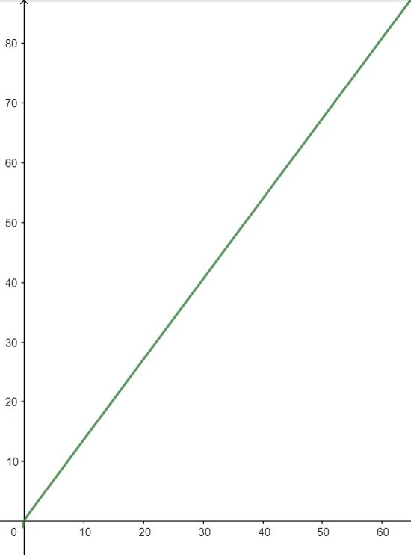
\includegraphics[width=6.906cm,height=9.3cm]{figures/Math_oraux-7.pdf}
  \caption{Graphe de la fonction $r \longmapsto \sqrt{95 r^2 + 75 r + 11} -
  \sqrt{41 r^2 + 33 r + 5} - 2 r - 1$}
\end{figure}


\

\

Donc, pour tout $n \geqslant 23 r^2 + 19 r + 3$, on a :
\[
\left( - (4r + 1) + \sqrt{4n + 3r^2 - r - 1} \right) - 
\left( - (2r + 1) + \sqrt{2n - 5r^2 - 5r - 1} \right) \geq 1
\]



Le probl{\`e}me est compl{\`e}tement r{\'e}solu.

\

Maintenant, pour aller plus loin et rendre ce probl{\`e}me plus difficile,
nous proposons les d{\'e}fis suivants :

\

\tmtextbf{Quelques d{\'e}fis.}

\tmtextbf{D{\'e}fi 1.}

$\star$ Soit $r > 1$ un entier, trouvez le plus petit entier $f (r)$ tel que,
pour tout $n \geqslant f (r)$, si l'on {\'e}crit les nombres $n, n + 1,
\ldots, 2 n$ chacun sur une carte diff{\'e}rente, puis que l'on m{\'e}lange
ces $n + 1$ cartes et qu'on les divise en deux tas, alors il existe $r$ cartes
dans l'un des tas dont la somme des nombres est un carr{\'e} parfait.

\

\tmtextbf{D{\'e}fi 2.}

$\star$ Soient $r, s > 1$ deux entiers. Trouvez le plus petit entier $g(r, s)$ tel que, pour tout $n \geqslant g(r, s)$, si l'on écrit les nombres $n, n + 1, \ldots, n + s$ chacun sur une carte diff{\'e}rente, puis que l'on
m{\'e}lange ces $s + 1$ cartes et qu'on les divise en deux tas, alors il
existe $r$ cartes dans l'un des tas dont la somme des nombres est un carr{\'e}
parfait.

\

\tmtextbf{D{\'e}fi 3.}

$\star$ Soient $r, s, t, v, w > 1$ cinq entiers, trouvez le plus petit entier
$h (r, s, t, v, w)$ tel que, pour tout $n \geqslant h (r, s, t, v, w)$, si
l'on {\'e}crit les nombres $n, n + 1, \ldots, n + s$ chacun sur une carte
diff{\'e}rente, puis que l'on m{\'e}lange ces $s + 1$ cartes et qu'on les
divise en $t$ tas, alors il existe $v$ cartes dans l'un des tas dont la somme
des nombres est une puissance parfaite de $w$.